\chapter{HTTPS komunikácia}
HTTPS (Hypertext Transfer Protocol with Security) je kombináciou protokolu HTTP so sieťový zabezpečovacím protokolom SSL (Secured Sockets Layer). HTTP pracuje na najvyššej vrstve TCP/IP modelu -- na aplikačnej vrstve. Rovnako ako aj bezpečnostný protokol TLS (pracujúci ako spodná podvrstva aplikačnej vrstvy), ktorý šifruje HTTP správu pred prenosom a dešifruje správu po príchode.

HTTPS vytvára bezpečný kanál cez nezabezpečenú sieť. To zaisťuje primeranú ochranu pred odposluchmi a útokmi typu "man-in-the-middle" za predpokladu, že sa použijú adekvátne šifrovacie algoritmy a serverový certifikát je overený a dôveryhodný. 

HTTPS URL adresy začínajú reťazcom \uv{https://} a štandardne používajú port $443$, zatiaľ čo HTTP adresy začínajú \uv{https://} a štandardne používajú port $80$.

Servery a klienti komunikujú stále pomocou HTTP, ale cez zabezpečené pripojenie SSL, ktoré šifruje a dešifruje ich požiadavky a odpovede. Vrstva SSL má 2 hlavné účely:

\begin{itemize}
	\item overenie, či prebieha komunikácia so server, ktoré boli požiadavky určené
	\item uistite sa, že len server dokáže čítať to, čo klient posiela
	\item uistite sa, že len klient dokáže čítať to, čo server odpovedá
\end{itemize}

Dôležitým faktom je, že každý môže zachytiť každý jednu zo správ, ktoré si klient vymenia so serverom, vrátane tých, v ktorých súhlasíte s kľúčovou a šifrovacou stratégiou, ktorú budete používať, no napriek tomu nikto nebude môcť prečítať žiadne odosielané údaje.

Pripojenie HTTPS sa používa pre webové aplikácie (napríklad on-line bankovníctvo), ktoré vyžadujú zabezpečené pripojenia na ochranu citlivého obsahu. Tradičné bezpečnostné zariadenia nemôžu dešifrovať a preskúmať tento obsah, vírus / škodlivý softvér a ďalšie hrozby zabudované v prevádzke protokolu HTTPS môžu prejsť bezproblémovo prostredníctvom bezpečnostnej ochrany a dostať sa do podnikovej siete.

HTTPS je obzvlášť dôležitá pri nezabezpečených sieťach (ako sú verejné prístupové body Wi-Fi), pretože každý v rovnakej lokálnej sieti môže odchytávať pakety a nájsť citlivé informácie, ktoré nie sú chránené protokolom HTTPS.

Nasadenie protokolu HTTPS tiež umožňuje používanie protokolu HTTP/2, ktorý je novou generáciou protokolu HTTP, určeného na zníženie času načítania stránok a latencie.

\chapter{Dešifrovanie HTTPS}

Na dešifrovanie HTTPS komunikácie postačia dva nástroje: webový prehliadač a nástroj Wireshark\footnote{\url{https://www.wireshark.org/}}. Nasledovný návod je určený pre OS Linux a bol otestovaný na Ubuntu Mate 17.10. Dešifrovanie HTTPS bude demonštrované na HTTPS stránke \url{http://wis.fit.vutbr.cz/} s IPv4 adresou $147.229.9.21$.

Nástroj Wireshark je nutné spustiť s root právami a začať odchytávať pakety. Je možné nastaviť filter $ip.src == 147.229.9.21$ pre jednoduchšie hľadanie skúmaných paketov. Následne je potrebné otvoriť webový prehliadač a otvoriť adresu \url{http://wis.fit.vutbr.cz/}. Záznamy paketov zachytených vo Wiresharku môžu vyzerať nasledovne:

\begin{figure}[h]
	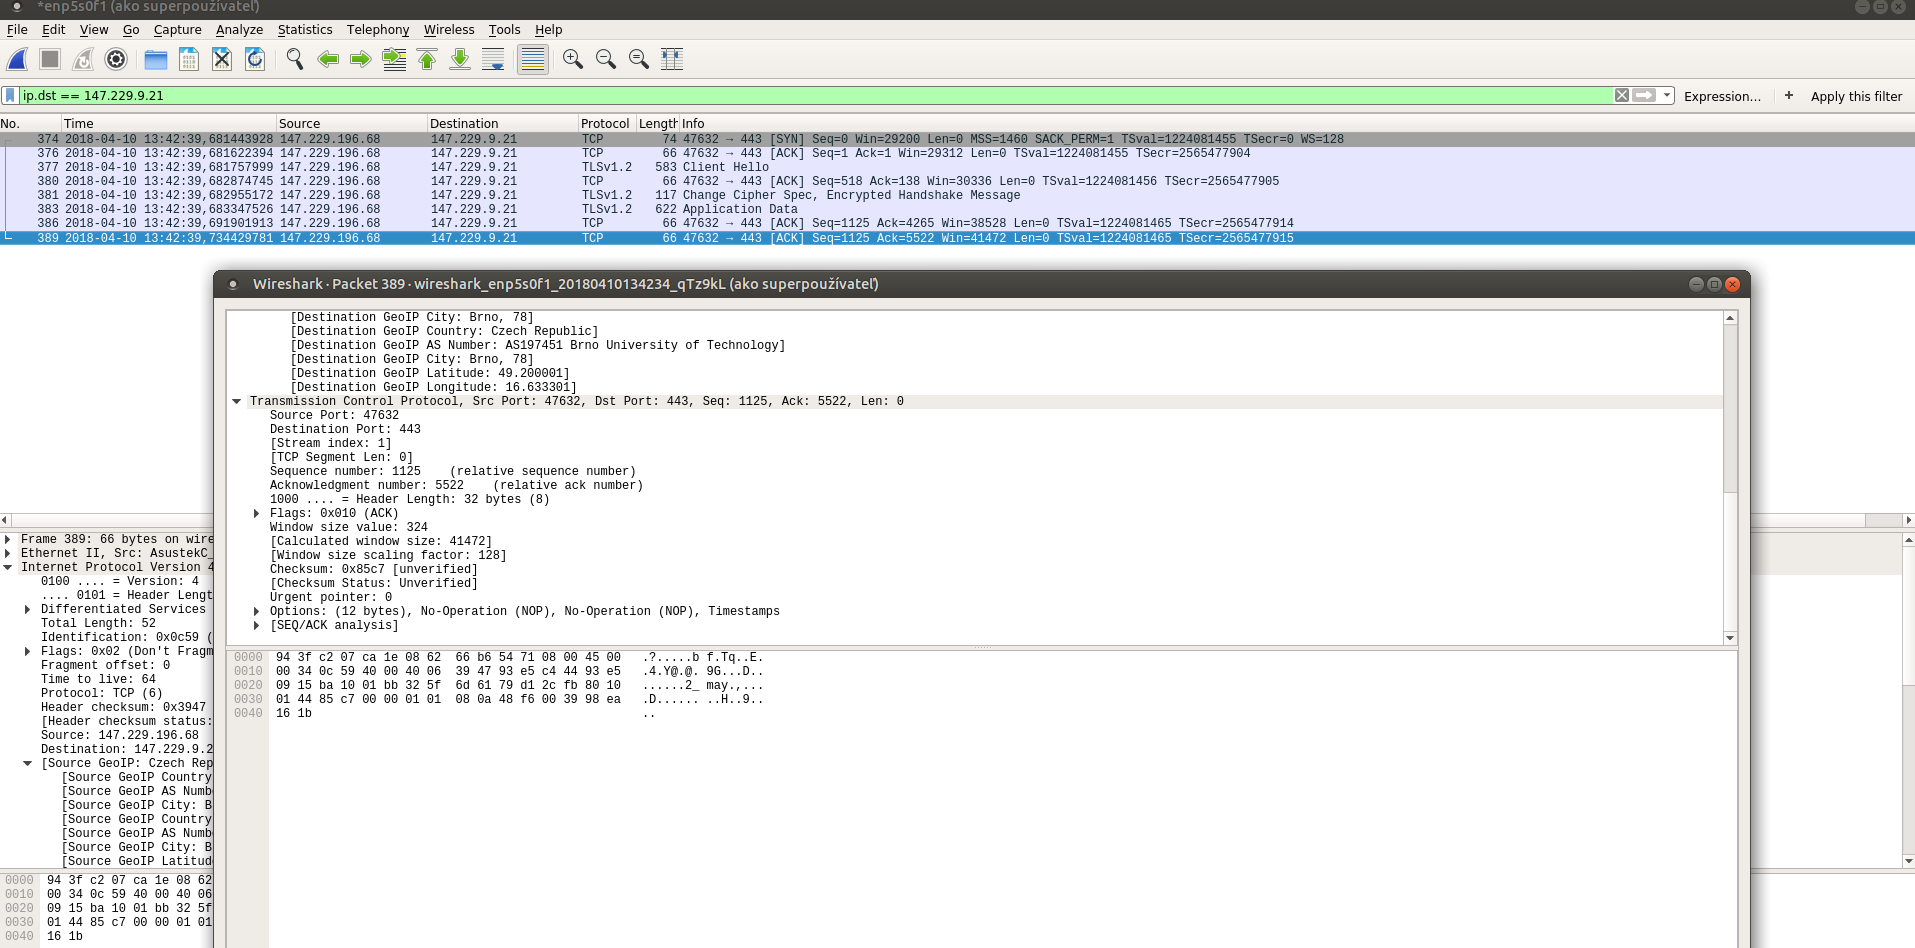
\includegraphics[width=\textwidth]{nodecrypt}
	\caption{Zašifrovaná HTTPS komunikácia}
\end{figure}

Pre dešifrovanie HTTPS komunikácie je možné použiť nasledovný postup. Vytvorím prázdny súbor pre záznamy obsahujúce odchytenú SSL komunikáciu. Pre túto demonštráciu som použil \textit{/home/xbolva00/ssl.log}. Otvorím Wireshark - Edit - Preferences - Protocols - SSL. Do pola \textit{(Pre)Master-Secret log filename} zadám cestu k súboru, ktorý som vytvoril -- \textit{/home/xbolva00/ssl.log}.

\pagebreak

Ďalej je potrebné spustiť príkaz
\textit{export SSLKEYLOGFILE=/home/xbolva00/ssl.log\textit} a následné z terminálu spustiť webový prehliadač a znova otvoriť HTTPS adresu \url{http://wis.fit.vutbr.cz/} a prihlásiť sa do IS FIT. Je vhodné znova nastaviť filter $ip.src == 147.229.9.21$ pre jednoduchšie hľadanie dešifrovaných paketov. Výstup vo Wireshark je nasledovný:

\begin{figure}[h]
	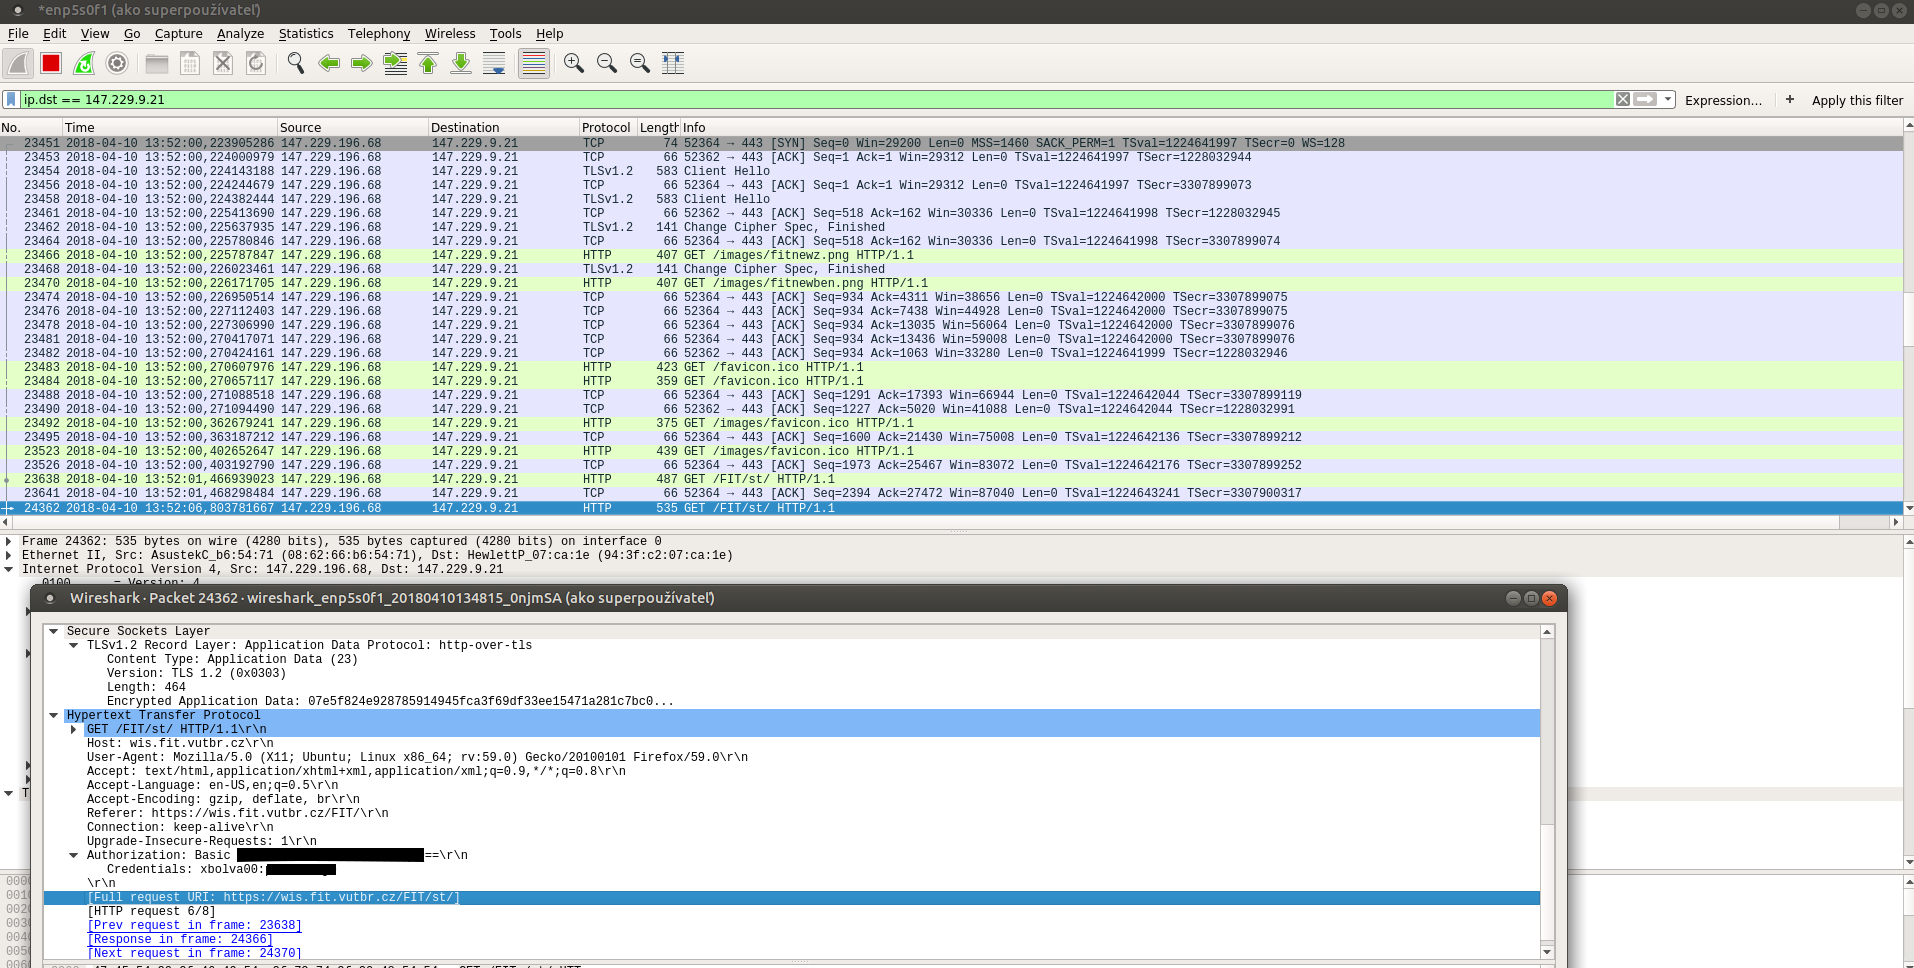
\includegraphics[width=\textwidth]{decrypt}
	\caption{Dešifrovaná HTTPS komunikácia}
\end{figure}

Ako je možné vidieť, HTTPS komunikácia bola dešifrovaná a vo Wiresharku je možné vidieť obsah, ktoré si klient so serverom posielal. Taktiež heslo prenášané v poli \textit{Authorization} je teraz zobrazované a môže byť zneužité na neoprávnený prístup do systému.


\chapter{Zhodnotenie}

V tejto práci bol prezentovaný postup ako dešifrovať zabezpečenú HTTPS komunikáciu za pomoci nástroja Wireshark. Využitie tohto dešifrovania možno hľadať v analýze samotnej komunikácie s rôznymi webovými stránkami.

Okrem zjavného škodlivého využitia má dešifrovanie SSL aj ďalšie možné využitia:

\begin{itemize}
	\item Ladenie aplikácií, ktoré používajú protokol SSL (HTTP, SMTP, POP3, IMAP, FTP atď.).
	\item Použitie dešifrovanej prevádzky pre IDS. Najlepšie podpisy na svete nepomôžu, ak všetky snímače vidia šifrovanú prevádzku.
	\item Pochopenie princípu fungovania SSL.
\end{itemize}

Z dešifrovanej prevádzky je možné zistiť, aké dáta prichádzajú a odchádzajú a tieto znalosti je možné využiť napríklad pre účely tvorby automatizačných skriptov, ktoré využívajú znalosti získané z tejto analýzy: môže ísť o odhalenie skrytých, neverejných API stránok, prípadne získanie tajných API kľúčov.